% Cut-off radius

\section{Gravity}

You probably know that Newtonian gravitational forces obey an inverse-square
law, with the force of object $i$ on object $j$ given by
\begin{equation*}
  F(\mathrm{r}_{ij}) = -G \frac{m_i m_j}{r_{ij}^2}\ 
                          \frac{\mathbf{r}_{ij}}{r_{ij}},
\end{equation*}
with $\mathbf{r}_{ij}$ standing for the vector going from $i$ to $j$, $m_i$ and 
$m_j$ the masses, $r_{ij}$ the distance from $i$ to $j$, and $G$ the universal
gravitational constant.

\begin{figure}
  \begin{center}
  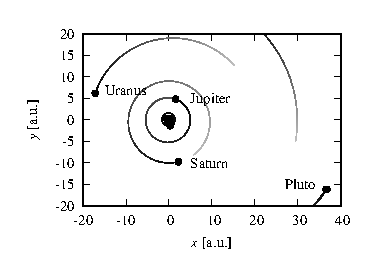
\includegraphics[width = 0.53\textwidth]{figures/gravity.eps}
  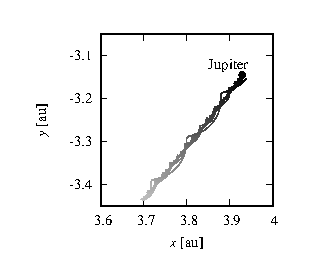
\includegraphics[width = 0.44\textwidth]{figures/Jupiter.eps}
  \end{center}
  \caption{\label{gravity}Motion of objects in the solar system for $10^4$ days 
           starting on the 10th of March 2021, when the code was run. In a 
           close-up of part of the trajectory for Jupiter (\textit{right}), you 
           can also see the trajectories of some of its moons.}
\end{figure}


